\chapter{实验方法和实验结果}

\zadd{本章首先介绍实验方法,包括实验工具链,实验平台和benchmark。然后介绍和分析实验结果,包括硬件属性分析,性能分析和能耗分析。最后我们对加速器的一些特性,如熵编码/解码,稀疏利用率等进行深入讨论。
}

\section{实验方法}
我们使用Synopsys工具链中的TMSC $65nm$库对加速器的RTL实现进行综合。我们使用CACTI 6.0预测DRAM访存能耗~\cite{muralimanohar2007optimizing}。我们使用基于PrimeTime PX的VCD波形文件评估能耗。最后我们使用基于事件触发的模拟器评估加速器的性能。

\subsection{Baseline}
我们将Cambricon-S与CPU,GPU和硬件加速器进行比较。

\subsubsection{CPU}
我们使用目前流行的深度学习框架Caffe~\cite{jia2014caffe}评估神经网络在CPU上的性能。CPU的型号是拥有6核的英特尔志强 E5-2620 v2,工作频率为$2.1GHz$,工艺为$22nm$。同时,我们使用稀疏库(sparse-BLAS)~\cite{duff2002overview}来评估稀疏神经网络的性能。我们用CPU-Caffe和CPU-Sparse分别表示稠密网络和稀疏网络在CPU上的性能。

\subsubsection{GPU}
我们使用Caffe评估神经网络在GPU上的性能(用GPU-Caffe表示)。GPU的型号是Nvidia K20,拥有$5GB$ GDDR5,峰值能够达到$3.52TFlops$,工艺为$28nm$。同时我们使用cuBLAS来实现神经网络算法(用GPU-cuBLAS表示)。最后,我们使用先进的cuSparse库评估稀疏神经网络的性能(用GPU-Sparse表示)。

\subsubsection{硬件加速器}
我们将新型加速器与目前最先进的神经网络加速器DianNao和Cambricon-X进行性能比较。DianNao拥有很高的吞吐量,能够加速大多数的CNN和DNN。Cambricon-X是一个稀疏神经网络加速器,它能够利用稀疏特性提高性能同时降低能耗。我们选择Cambricon-X作为baseline,主要是考虑到它能够最大程度利用稀疏特性,并且具有通用性。考虑到稀疏利用率,对比稠密神经网络,Cambricon-X通过挖掘稀疏性能够获得2.93倍的加速比,而Cnvlutin和SCNN分别只能获得1.37倍和2.7倍的加速比。考虑到通用性,SCNN在全连接层上的性能非常低,而EIE只能用来加速稀疏的全连接层。

\subsection{Benchmark}
如表~\ref{tab:compression}所示,我们使用七个代表神经网络:AlexNet, VGG16, LeNet-5,MLP,Cifar10,ResNet152和LSTM作为benchmark。值得注意的是,我们表中参数都是经过粗粒度剪枝后的网络参数。

\section{实验结果}

\subsection{硬件属性}

在当前的加速器中,为了兼容剪枝块的大小,我们将PE的数量$T_n$以及每个PE内部乘法器数量$T_m$配置为$T_n = T_m = 16$,同时考虑到神经网络神经元和权值的稀疏度,我们将NSM设计为256选16的结构,SSM设计为64选16的结构,Encoder设计为64选16的结构。新型加速器的布局特点,各模块的面积和功耗如表~\ref{tab:hardware}所示。加速器的总面积和总功耗分别是$6.82mm^2$和$821.19mW$,工作频率为1GHz,吞吐量为512GOP/s,片上SRAM共为$54KB$。新型加速器的面积分别是Cambricon-X($6.38mm^2$)和DianNao($3.02mm^2$)的1.07倍和2.26倍,同时功耗比Cambricon-X($954mW$)低$132.81mW$,比DianNao($485mW$)高$336.19mW$。
值得注意的是,我们当前加速器并不包含熵解码模块,因此不支持经过熵编码后的神经网络。

\begin{table}[h]
\caption{加速器详细属性}
\centering
\label{tab:hardware}
\begin{tabular}{lllllllllllll}
\toprule
 & Area($mm^2$) & \% & Power(mW) & \% \\
\midrule
Total   & 6.82	& 100.00\% 	& 821.19    & 100.00\% \\
\midrule
NBin    & 0.55  & 8.06		& 93.32     & 11.36	\\
NBout   & 0.55  & 8.06	    & 93.32     & 11.36	\\
SIB     & 0.05 	& 0.73		& 6.89      & 0.84	\\
NIB     & 0.05  & 0.73      & 6.89      & 0.84  \\
CP      & 0.16 	& 2.35		& 75.06     & 9.14	\\
NSM     & 0.69 	& 10.12		& 121.46    & 14.79	\\
Encoder & 0.04  & 0.60      & 15.75     & 1.92  \\
NFU     & 4.73 	& 69.35 	& 408.50    & 49.75	\\
~~~SB   & ~~~1.05 	& ~~~22.20	& ~~~151.91 & ~~~37.19\\
~~~SSM  & ~~~0.25 	& ~~~5.29	& ~~~56.80  & ~~~13.90	\\
~~~WDM  & ~~~1.54 	& ~~~32.56	& ~~~16.25  & ~~~3.98	\\
~~~PEFU & ~~1.89	& ~~~33.95	& ~~~183.54 & ~~~44.93 \\
\bottomrule
\end{tabular}
\end{table}

此外,Cambricon-S中处理稀疏和量化模块(NSM, SSMs, Encoder和WDM)的面积和功耗分别是$2.52mm^2$(占总面积的$36.95\%$)和$210.26mW$(占总功耗的$25.60\%$),却能够获得比Cambricon-X高的1.71倍性能,同时降低1.75倍的能耗。值得注意的是,即使新增了突触选择模块,新型加速器的索引模块(即NSM和SSM)的面积对比与Cambricon-X的IM模块减少了2.11倍($0.94mm^2$ vs. $1.98mm^2$),功耗减少了1.87 倍($178.26mW$ vs. $332.62mW$);同时新型加速器的NSM的面积和功耗分别是Cambricon-X中IM模块的$36.52\%$和$34.85\%$,却实现了与IM模块相同的功能(即筛选神经元)。因此,我们的设计对比于Cambricon-X在面积,能耗上都有很大的提升。

\subsection{性能}
在表~\ref{tab:compression}所列出的七个benchmark上,我们比较了Cambricon-S,CPU,GPU,DianNao和Cambricon-X的性能。在CPU和GPU上,我们同时评估稀疏神经网络和稠密神经网络的性能,即我们使用稀疏库(CPU-Sparse,GPU-Sparse)评估稀疏神经网络的性能,使用稠密库(CPU-Caffe, GPU-Caffe, GPU-cuBLAS)评估稠密神经网络的性能。为了与CPU和GPU公平比较,我们评估了加速器在稠密网络上的性能(ACC-dense)。同时为了与Cambricon-X和DianNao公平比较,我们评估了这三个加速器在稀疏神经网络上的性能。

\begin{figure}[h]
\centering
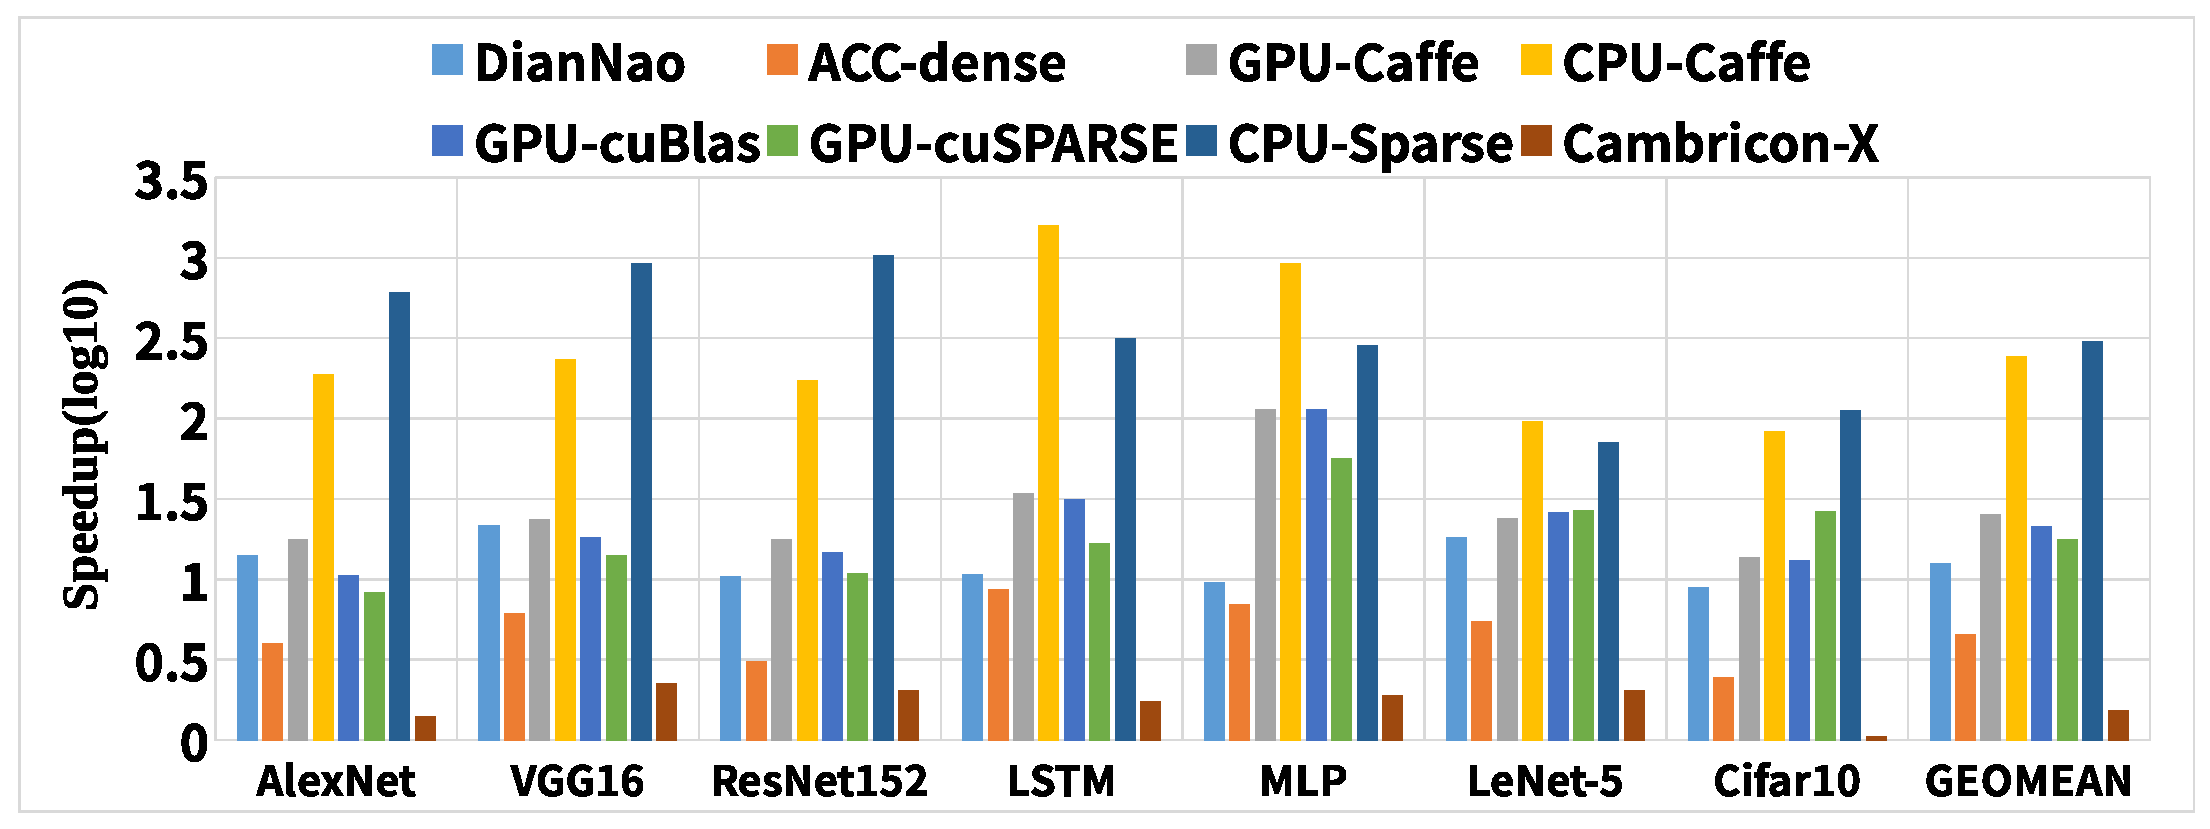
\includegraphics[width=0.8\columnwidth]{total_performance.eps}
\caption{Cambricon-S与CPU,GPU,DianNao,Cambricon-X的性能对比}
\label{fig:total_performance}
\end{figure}

在图~\ref{fig:total_performance},我们比较了Cambricon-S,CPU,GPU,DianNao和Cambricon-X的性能,同时,我们将所有性能的数据归一化到了Cambricon-S在稀疏网络上的性能。在稠密网络上,Cambricon-S与CPU-Caffe,GPU-Caffe和CPU-cuBLAS对比分别能够获得44.8倍,5.8倍和5.1倍的加速比。在稀疏网络上,Cambricon-S与CPU-Sparse和GPU-cuSparse对比分别能够获得331.1倍和19.3倍的加速比。对比于DianNao和Cambricon-X,Cambricon-S分别能够获得13.10倍和1.71倍加速的加速比。实验结果充分显示了我们的加速器能够充分利用利用神经网络稀疏的特性,从而获得高加速比。值得注意的是,我们的加速器能够通过关闭/开启各个模块(NSM,SSM,WDM,Encoder等),使得加速器能够处理稠密神经网络,稀疏神经网络(包括只利用权值稀疏,只利用神经元稀疏和同时利用神经元/权值稀疏三种情况),局部量化。

为了进一步探索Cambricon-S的性能,我们统计了Cambricon-S在卷积层和全连接层上的性能。如图~\ref{fig:conv_performance}所示,在卷积层上,对比于CPU-Sparse, GPU-cuSparse和DianNao,我们的加速器分别获得了283.31倍,12.20倍和13.94倍的性能提升。如图~\ref{fig:fc_performance}所示,在全连接层上,对比于CPU-Sparse, GPU-cuSparse和DianNao,我们的加速器分别获得了531.89倍,79.05倍和13.56倍的性能提升。值得注意的是,对比于Cambricon-X,Cambricon-S能够在卷积层和全连接层分别获得1.66倍和2.15倍的加速比。

\begin{figure}[h]
\centering
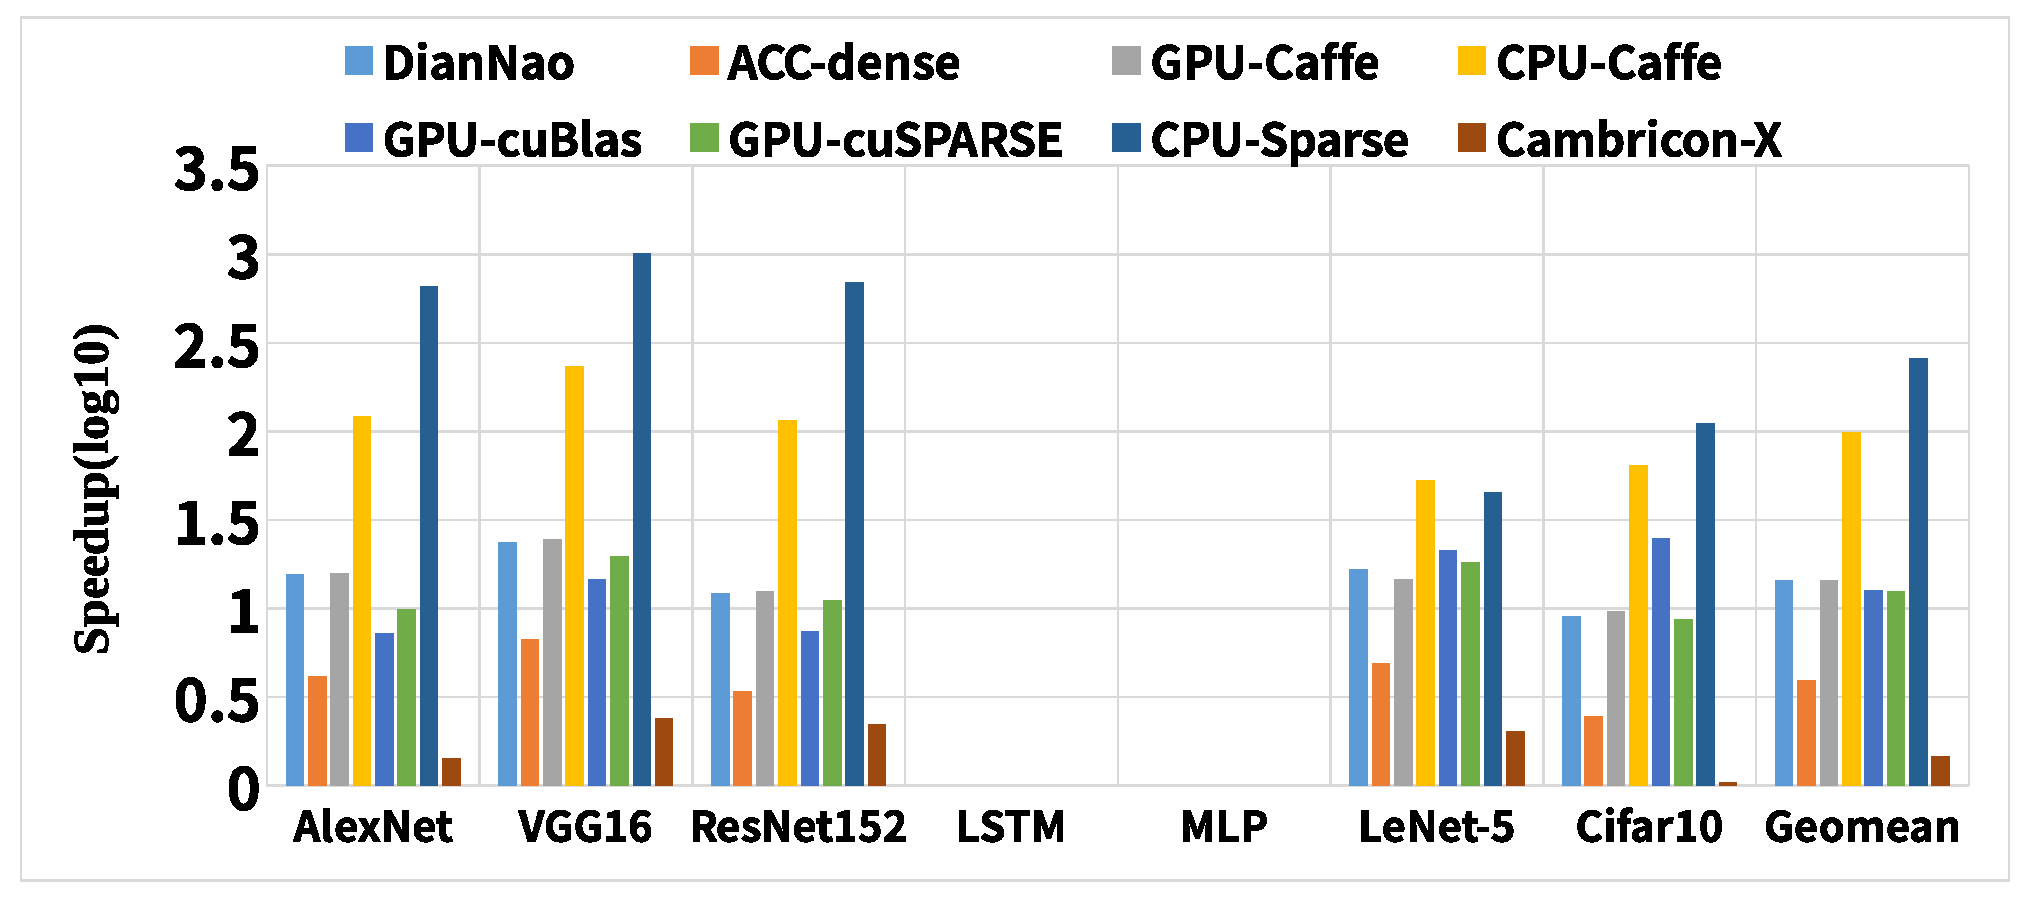
\includegraphics[width=0.8\columnwidth]{conv_performance.eps}
\caption{Cambricon-S与CPU,GPU,DianNao,Cambricon-X在卷积层上的性能对比}
\label{fig:conv_performance}
\end{figure}

\begin{figure}[h]
\centering
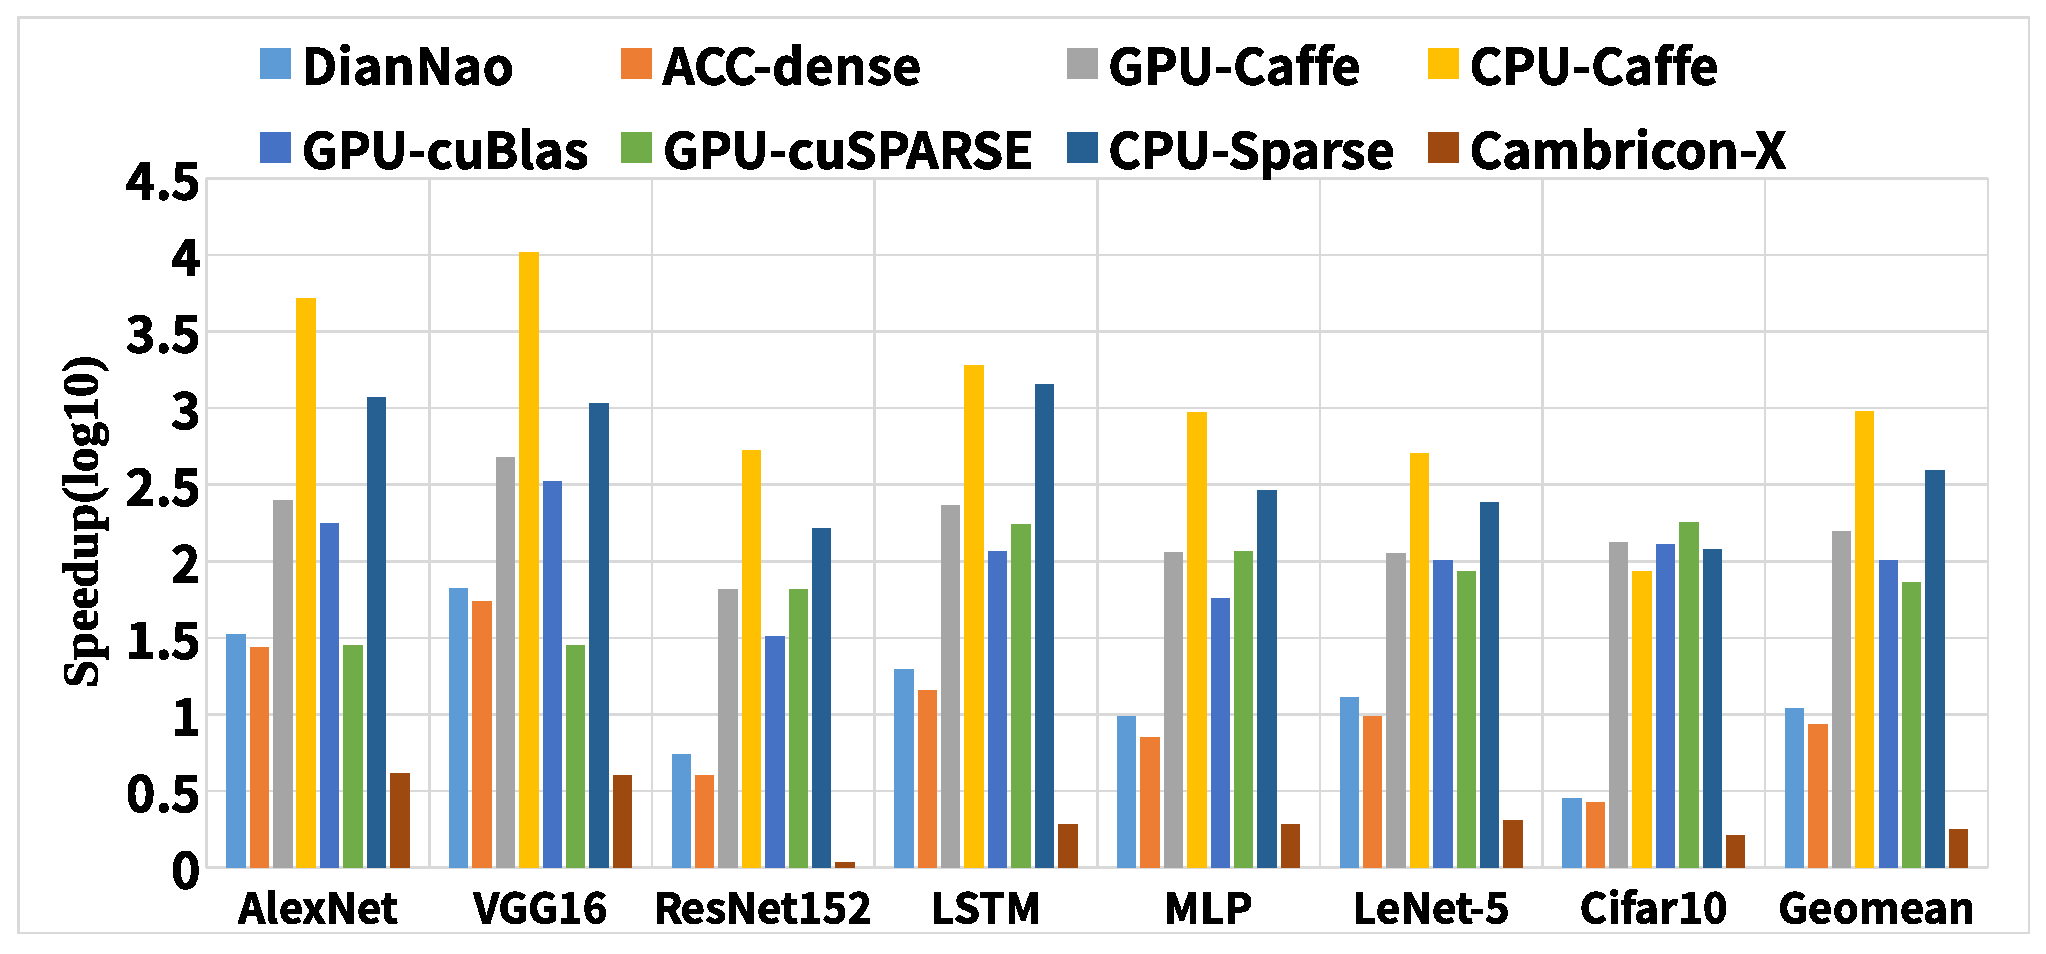
\includegraphics[width=0.8\columnwidth]{fc_performance.eps}
\caption{Cambricon-S与CPU,GPU,DianNao,Cambricon-X在全连接层上的性能对比}
\label{fig:fc_performance}
\end{figure}


在卷积层上的性能主要来源于SSM模块能够进一步挖掘神经元稀疏,因为卷积层是计算密集型的层,动态神经元稀疏可以大量减少神经网络中的计算量,例如在AlexNet网络的\emph{conv3}层,稠密情况下需要$52M$的MAC操作(Multiply–accumulate operation),而如果利用$45\%$的动态神经元稀疏,仅仅需要$29M$的MAC操作。

在全连接层的性能提升主要来源于权值存储量的减少(局部量化)和索引存储量的减少(索引共享)。WDM能够支持用户自定义比特长度的量化,从而减少突触的存储容量,获得1.77倍的加速比;粗粒度剪枝使得非零位置的索引信息能够被相邻多个输出神经元共享,因此能够额外获得1.21倍的加速比。


\subsection{能耗}
\begin{figure}[h]
\centering
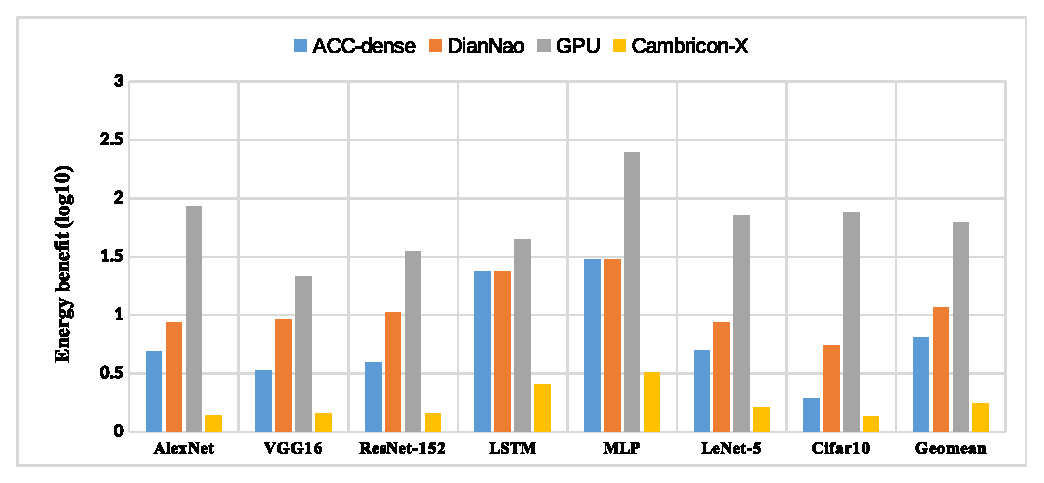
\includegraphics[width=0.8\columnwidth]{energy.eps}
\caption{新型加速器与GPU,DianNao,Cambricon-X在能耗的对比}
\label{fig:energy}
\end{figure}

\zadd{在七个benchmark上,我们比较了Cambricon-S,GPU,DianNao和Cambricon-X的能耗,其中我们包括了片外访存的能耗。如图~\ref{fig:energy}所示,对比于GPU,DianNao和Cambricon-X,Cambricon-S能够分别节约63.49倍,11.72倍和1.75倍的能耗。此外,我们观察到局部量化能够节约1.24倍的能耗,动态压缩神经元能够节约1.28倍的能耗。如果不考虑片外访存的能耗,Cambricon-S分别比GPU,DianNao和Cambricon-X节约1169.51倍,12.30倍和1.75倍能耗。以上实验数据证明我们的加速器能够使用很低的能耗完成神经网络的运算。
}


\begin{figure}[h]
\centering
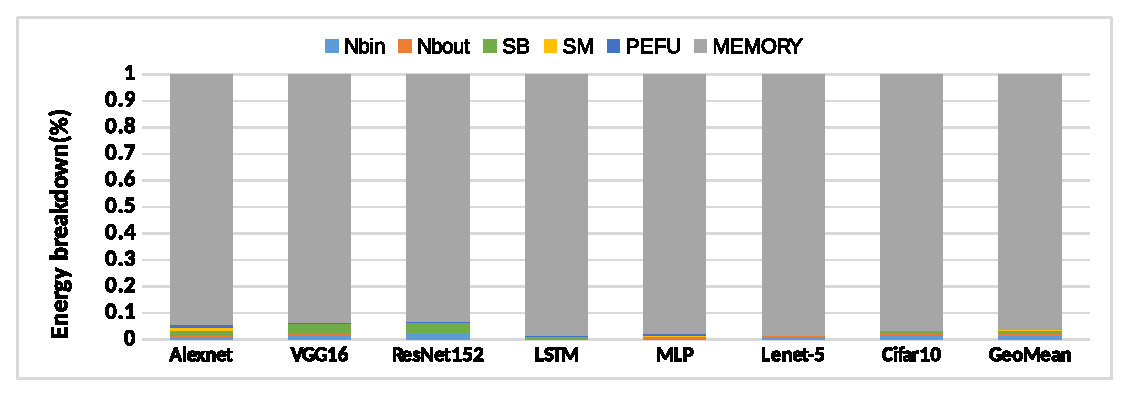
\includegraphics[width=0.8\columnwidth]{energy_breakdown.eps}
\caption{加速器在benchmark上的能耗分布(包括片外访存能耗)}
\label{fig:energy_breakdown}
\end{figure}

我们分析了加速器在七个benchmark上的能耗分布。如图~\ref{fig:energy_breakdown}所示,我们可以观察到片外访存消耗了超过$90\%$的总能量。在LSTM和MLP网络中,这个比例高达$98\%$,远高于其他神经网络,因此这两个网络是访存密集型的网络。实验结果显示,通过稀疏和量化可以显著减少片外访存的能耗。对比于稠密网络,稀疏网络能够减少$72.6\%$的片外访存能耗。

\begin{figure}[h]
\centering
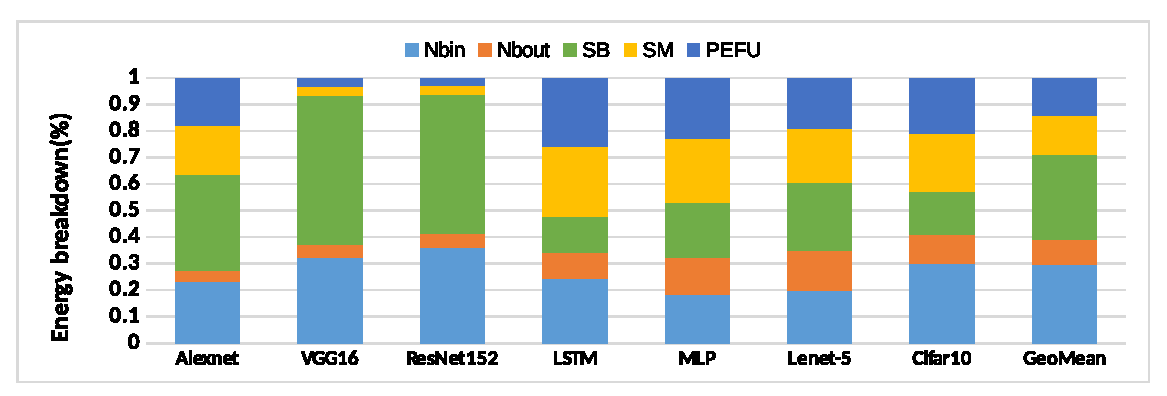
\includegraphics[width=0.8\columnwidth]{energy_breakdown2.eps}
\caption{加速器在benchmark上的能耗分布(不包括片外访存能耗)}
\label{fig:energy_breakdown2}
\end{figure}

我们进一步分析了在不包括片外访存能耗情况下加速器的能耗分布。如图~\ref{fig:energy_breakdown2}所示,片上缓存访问能耗(包括NBin,NBout和SB)平均消耗约$70\%$的总能量,这表明片上缓存访问能耗依然主导片上的能耗。对于LSTM和MLP这两个网络上,片上缓存能耗少于$60\%$,因为在这两个网络中权值不进行重用。对于深层的卷积网络,比如VGG16和ResNet152,片上内存访问能源的比例超过$90\%$,因为在这两个网络中需要复杂的loop tiling和数据重用策略将大规模运算映射到加速器熵。值得注意的是,与Cambricon-X相比,局部量化能够减少2.76倍的权值存储量,从而使得SB节约2.48倍的能耗。

\section{讨论}

\subsection{熵编码和熵解码模块}

目前Cambricon-S中并没有加入熵解码模块(entropy decoding module)来支持权值熵编码,主要是考虑到熵解码模块需要耗费非常大的面积和能耗,但是仅仅能够获得非常有限的性能提升。一个熵解码模块(entropy decoding module)的面积为$6.781*10^{-3}mm^2$,它能够在一个cycle解码出一个码字。由于熵编码是一种变长编码,因此对应的解码模块必须串行进行解码。即使我们可以将数据划分为许多并行的数据流,然后为每个数据流提供一个熵解码模块,这种方法将会引入巨大的面积和能耗开销。

考虑到每一个SB需要在一个cycle提供$T_m\times 4$个数据,为了避免性能损失,我们必须为一个SB提供$T_m\times 4$个熵解码模块,因此我们的加速器总共需要集成$T_n\times T_m\times 4$个熵解码模块。在$T_m = T_n = 16$的配置下,我们总共需要1024个熵解码模块,这将引入额外$6.94mm^2$的面积和$971.37mW$的功耗,因此加速器的总面积和功耗分别是$13.67mm^2$和$1769.92mW$,分别是原始设计的2.03倍和2.22倍。然而,新增熵解码的加速器在卷积层上几乎没有性能提升,在全连接层也只有1.18倍的性能提升,对比与额外的面积和功耗开销,这种性能提升是非常有限的。因此,我们在加速器中不加入熵解码模块。

\subsection{稀疏度与性能}
\begin{figure}[h]
\centering
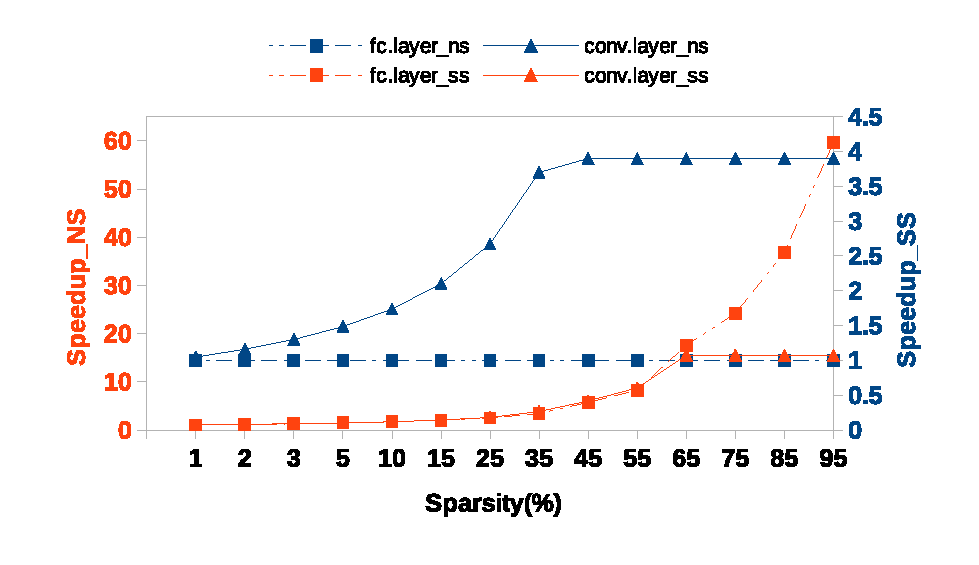
\includegraphics[width=0.8\columnwidth]{sensitivity.eps}
\caption{神经网络稀疏度对加速器性能的影响}
\label{fig:sensitivity}
\end{figure}

我们研究了Cambricon-S对神经网络稀疏度的敏感性,即稀疏度对神经网络性能的影响。如图~\ref{fig:sensitivity}所示,我们分别探究了神经元稀疏度和粗粒度权值稀疏度对加速器性能的影响,更进一步的,我们从卷积层和全连接层两个角度进行探究。从图中的数据我们观察到了几个有趣的实验结果:

1)考虑粗粒度权值稀疏,加速器能够在卷积层获得接近理想值的加速比(15.5倍 vs. 16倍)。为了兼容大多数网络的权值稀疏度(如表~\ref{tab:sparsities}所示),我们将NSM设计成为256选16的结构,即NSM最多从256个输入神经元中筛选出16个需要进行计算的神经元,从而最多实现16倍的加速器。我们的加速器能够接近理想加速器的主要原因是我们使用乒乓的模式管理片上缓存,使得加速器的片外访存延迟能够被运算时间覆盖。值得注意的是,由于我们的加速器能够充分利用粗粒度稀疏实现负载均衡,因此在相同稀疏度情况下,Cambricon-S能够获得比Cambricon-X更优的加速比。

2)考虑粗粒度权值稀疏,在全连接层中,Cambricon-S能够很容易地在低稀疏度情况下(低于$5\%$)获得加速比,并且随着稀疏度的提高,加速比也会不断提高,在稀疏度为$99\%$时能够获得59.59倍的加速比。主要原因是全连接层是一个访存密集的层,稀疏权值能够大大减少片外访存数据量,从而减少片外访存时间,减少总执行时间。

3)考虑神经元稀疏,Cambricon-S在卷积层最高能够获得3.9倍的加速比,接近理想的4倍加速比。由于在大多数情况下,神经元的稠密度高于$25\%$(稀疏度低于$75\%$),我们将SSM设计成为64选16的结构,因此最多获得4倍的加速比。这个设计能够满足绝大多数神经网络的需求。

4)神经元稀疏并不能在全连接层带来性能的提升,因此在全连接层片外权值访存时间主导了总执行时间(超过$99\%$),而神经元稀疏并不能有效地减少内存访问。

上述的实验结果进一步验证了我们的加速器能够高效地利用神经网络中神经元稀疏和权值稀疏。

\subsection{减少的不规则度}
减少稀疏神经网络的不规则度能够对加速器的设计,性能产生深远的影响。第一,减少不规则度能够简化加速器的设计。我们可以使用一个共享的NSM取代$T_n$个分布式的NSM,从而节省$10.35mm^2$的面积和$1821.9mW$的功耗;同时我们可以用一个共享的SIB来代替16个独立的SIB,从而节省$15KB$的SRAM大小。第二,减少不规则度能够大大减少权值索引的规模(26.83倍),减少片外访问权值,从而获得1.06倍的加速比,节约1.11倍的能耗。

\subsection{类似粗粒度稀疏的方法}
最近有不少类似于粗粒度稀疏的研究,例如SIMD-aware weight pruning~\cite{yu2017scalpel},synapse vector elimination~\cite{hill2017deftnn},channel reduction和filter reduction~\cite{wen2016learning,lebedev2016fast}。尽管这些技术可以减少稀疏神经网络的不规则度,从而简化加速器设计,但是通常会导致显著的精度损失~\cite{li2016pruning}。

\citet{mao2017exploring}探究了一系列结构化稀疏的方法,包括细粒度稀疏(fine-grained sparsity),向量层次稀疏(vector-level sparsity),卷积核层次稀疏(kernel-level sparsity)和过滤器层次稀疏(filter-level sparsity),同时评估这些稀疏方法对神经网络不规则度和精度的影响。 值得注意的是,我们提出的粗粒度剪枝方式并不会限制剪枝块的规模,因此是一种普遍性的剪枝方法。通过指定参数,粗粒度剪枝能够达到上述各种形式稀疏的效果。

\subsection{其他稀疏神经网络加速器}
EIE~\cite{han2016eie}能够加速稀疏神经网络的全连接层,它采用CSC的压缩方式压缩权值。为了能够完全消除片外访存,它使用非常大的片上缓存存储所有的突触。为了使AlexNet网络的全连接层权值能够完全存储在片上缓存,EIE的总面积需要达到$40.8mm^2$,是我们加速器的面积的5.07倍。同时,EIE只支持固定比特的量化,而新型加速器中的WDM能够支持自定义比特的量化,从而权衡神经网络的压缩效果和精度。为了公平地与EIE比较性能,我们假设加速器的片上缓存足够大,能够存储全连接层的所有权值,因此我们将加速器的性能聚焦在计算时间。如表~\ref{tab:EIE}所示,相比于EIE,新型加速器能够平均获得1.65倍的加速比。

\begin{table}[h]
\centering
\caption{\footnotesize Cambricon-S与EIE的性能比较 \emph{(microsecond)}.}
\label{tab:EIE}
\begin{tabular}{@{}lll@{~~}lll@{~~}lll@{~~}lll@{~~}lll@{~~}lll@{~~}lll@{~~}lllllll}
\toprule
layer & \multicolumn{3}{c}{AlexNet} & \multicolumn{3}{c}{VGG16} & Geomean\\
& fc6 & fc7 & fc8 & fc6 & fc7 & fc8     \\
\midrule
EIE & 30.30 & 12.20 & 9.90  & 34.40 & 8.70  & 7.50  & --\\
ACC & 18.43 & 8.19  & 5.13  & 25.23 & 4.12  & 5.09  & --\\
Speedup & $1.64\times$ & $1.49\times$ & $1.93\times$ & $1.36\times$ & $2.11\times$ & $1.49\times$ & $1.65\times$ \\
\bottomrule
\end{tabular}
\end{table}

我们的加速器与Cambricon-X~\cite{zhang2016cambricon}都是用了索引的方式利用神经网络的稀疏性质,但是Cambricon-S索引方式与Cambricon-X有三个方面不同。首先,Cambricon-S包含一个共享的索引模块(NSM),它能够充分挖掘权值的粗粒度稀疏特性。由于粗粒度稀疏,加速器的各个PE共享相同的索引,因此NSM筛选出的神经元能够被PE共享,从而减少索引模块开销以及NSM与PE之间的带宽需求。第二,Cambricon-S的PE中集成了一个本地的权值索引模块(SSM),从而充分利用神经元稀疏。虽然粗粒度稀疏能够减少稀疏神经网络的不规则性,但是稀疏的神经元依然存在不规则性,例如ReLU激励能够使得许多神经元的激励为“0”,SSM模块能够最小化这种不规则性的影响。因此新型索引模块能够充分利用神经元稀疏和权值稀疏,而Cambricon-X只能利用权值稀疏。第三,Cambricon-S中集成了Encoder模块,动态压缩稀疏的神经元,从而减少片外神经元访问。实验显示,Encoder模块能够进一步节约1.28倍的能耗;更具体地说,它能够在卷积层和全连接层分别节约1.68倍和1.02倍的能耗。第四,Cambricon-S的每一个PE中集成了WDM模块用于解码量化后的权值,从而充分利用局部量化,进一步减少片外权值访问量。

\zadd{SCNN~\cite{angshuman2017scnn}能够挖掘权值稀疏和神经元稀疏,对比于稠密神经网络,它能够获得2.7倍的加速比,同时节约2.3倍的能耗。而我们加速器能够获得4.32倍的加速比,节约6.53倍的能耗,这充分显示了我们加速器高性能和低能耗的特点。Cambricon-S在处理稀疏神经网络时能够获得4.32倍的加速比,这部分的性能提升主要来自于三个方面。首先,NSM可以充分利用突触稀疏(平均权值稀疏度为$87.99\%$)从而减少计算,最终实现2.06倍的加速比。第二,SSM能够充分利用神经元稀疏(平均神经元稀疏度为$55.41\%$),从而减少神经网络所需的计算量,最终获得1.44倍的加速比。第三,粗粒度稀疏($78.99\%$)和局部量化(减少2.76倍突触数据)可以大大减少片外权值访问量,从而获得1.46倍的加速比。
}

\section{本章小结}
\zadd{在本章,我们评估了Cambricon-S的性能和能耗。}
    
\zadd{我们首先介绍了实验工具链,实验平台,baseline和benchmark。在$65nm$工艺下,Cambricon-S的面积和功耗仅仅为$6.82mm^2$和$821.19mW$。
我们在七个benchmark上分别比较了CPU,GPU,DianNao,Cambricon-X和Cambricon-S的性能和能耗,我们发现Cambricon-S具有高性能和低能耗的特点。与最先进的稀疏的神经网络加速器Cambricon-X相比,Cambricon-S能够获得1.71倍的加速比,同时节约1.75倍的能耗。
}

\zadd{
最后,我们详细讨论了Cambricon-S的一些特性,我们发现在加速器中集成熵解码模块会耗费非常大的面积和能耗,但是不能获得非常理想的性能提升,因此我们不在加速器中集成熵解码模块。同时,我们发现加速器能够高效地利用神经网络中神经元稀疏特性和权值稀疏特性,且对稀疏特性的利用率高于Cambrcion-X,EIE和SCNN。}


